\chapter{The Accusation}

M. d’Avrigny soon restored the magistrate to consciousness, who had
looked like a second corpse in that chamber of death.

“Oh, death is in my house!” cried Villefort.

“Say, rather, crime!” replied the doctor.

“M. d’Avrigny,” cried Villefort, “I cannot tell you all I feel at this
moment,—terror, grief, madness.”

“Yes,” said M. d’Avrigny, with an imposing calmness, “but I think it is
now time to act. I think it is time to stop this torrent of mortality.
I can no longer bear to be in possession of these secrets without the
hope of seeing the victims and society generally revenged.”

Villefort cast a gloomy look around him. “In my house,” murmured he,
“in my house!”

“Come, magistrate,” said M. d’Avrigny, “show yourself a man; as an
interpreter of the law, do honor to your profession by sacrificing your
selfish interests to it.”

“You make me shudder, doctor. Do you talk of a sacrifice?”

“I do.”

“Do you then suspect anyone?”

“I suspect no one; death raps at your door—it enters—it goes, not
blindfolded, but circumspectly, from room to room. Well, I follow its
course, I track its passage; I adopt the wisdom of the ancients, and
feel my way, for my friendship for your family and my respect for you
are as a twofold bandage over my eyes; well——”

“Oh, speak, speak, doctor; I shall have courage.”

“Well, sir, you have in your establishment, or in your family, perhaps,
one of the frightful monstrosities of which each century produces only
one. Locusta and Agrippina, living at the same time, were an exception,
and proved the determination of Providence to effect the entire ruin of
the Roman empire, sullied by so many crimes. Brunhilda and Fredegund
were the results of the painful struggle of civilization in its
infancy, when man was learning to control mind, were it even by an
emissary from the realms of darkness. All these women had been, or
were, beautiful. The same flower of innocence had flourished, or was
still flourishing, on their brow, that is seen on the brow of the
culprit in your house.”

\begin{figure}[ht]
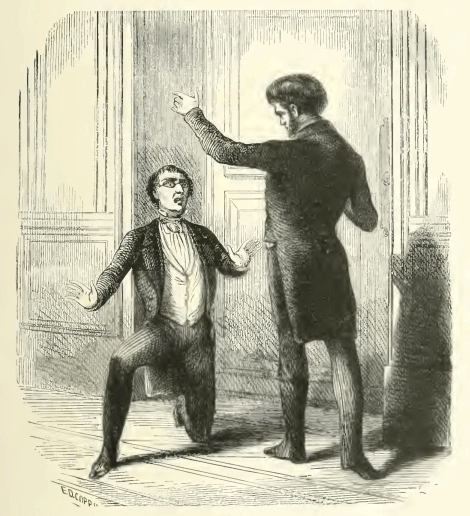
\includegraphics[width=\textwidth]{40120m.jpg}
\end{figure}

Villefort shrieked, clasped his hands, and looked at the doctor with a
supplicating air. But the latter went on without pity:

“‘Seek whom the crime will profit,’ says an axiom of jurisprudence.”

“Doctor,” cried Villefort, “alas, doctor, how often has man’s justice
been deceived by those fatal words. I know not why, but I feel that
this crime——”

“You acknowledge, then, the existence of the crime?”

“Yes, I see too plainly that it does exist. But it seems that it is
intended to affect me personally. I fear an attack myself, after all
these disasters.”

“Oh, man!” murmured d’Avrigny, “the most selfish of all animals, the
most personal of all creatures, who believes the earth turns, the sun
shines, and death strikes for him alone,—an ant cursing God from the
top of a blade of grass! And have those who have lost their lives lost
nothing?—M. de Saint-Méran, Madame de Saint-Méran, M. Noirtier——”

“How? M. Noirtier?”

“Yes; think you it was the poor servant’s life was coveted? No, no;
like Shakespeare’s Polonius, he died for another. It was Noirtier the
lemonade was intended for—it is Noirtier, logically speaking, who drank
it. The other drank it only by accident, and, although Barrois is dead,
it was Noirtier whose death was wished for.”

“But why did it not kill my father?”

“I told you one evening in the garden after Madame de Saint-Méran’s
death—because his system is accustomed to that very poison, and the
dose was trifling to him, which would be fatal to another; because no
one knows, not even the assassin, that, for the last twelve months, I
have given M. Noirtier brucine for his paralytic affection, while the
assassin is not ignorant, for he has proved that brucine is a violent
poison.”

“Oh, have pity—have pity!” murmured Villefort, wringing his hands.

“Follow the culprit’s steps; he first kills M. de Saint-Méran——”

“Oh, doctor!”

“I would swear to it; what I heard of his symptoms agrees too well with
what I have seen in the other cases.” Villefort ceased to contend; he
only groaned. “He first kills M. de Saint-Méran,” repeated the doctor,
“then Madame de Saint-Méran,—a double fortune to inherit.” Villefort
wiped the perspiration from his forehead. “Listen attentively.”

“Alas,” stammered Villefort, “I do not lose a single word.”

“M. Noirtier,” resumed M. d’Avrigny in the same pitiless tone,—“M.
Noirtier had once made a will against you—against your family—in favor
of the poor, in fact; M. Noirtier is spared, because nothing is
expected from him. But he has no sooner destroyed his first will and
made a second, than, for fear he should make a third, he is struck
down. The will was made the day before yesterday, I believe; you see
there has been no time lost.”

“Oh, mercy, M. d’Avrigny!”

“No mercy, sir! The physician has a sacred mission on earth; and to
fulfil it he begins at the source of life, and goes down to the
mysterious darkness of the tomb. When crime has been committed, and
God, doubtless in anger, turns away his face, it is for the physician
to bring the culprit to justice.”

\begin{figure}[ht]
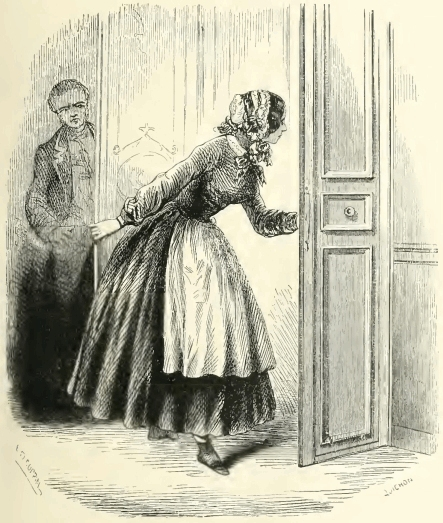
\includegraphics[width=\textwidth]{40122m.jpg}
\end{figure}

“Have mercy on my child, sir,” murmured Villefort.

“You see it is yourself who have first named her—you, her father.”

“Have pity on Valentine! Listen, it is impossible. I would as willingly
accuse myself! Valentine, whose heart is pure as a diamond or a lily!”

“No pity, procureur; the crime is fragrant. Mademoiselle herself packed
all the medicines which were sent to M. de Saint-Méran; and M. de
Saint-Méran is dead. Mademoiselle de Villefort prepared all the cooling
draughts which Madame de Saint-Méran took, and Madame de Saint-Méran is
dead. Mademoiselle de Villefort took from the hands of Barrois, who was
sent out, the lemonade which M. Noirtier had every morning, and he has
escaped by a miracle. Mademoiselle de Villefort is the culprit—she is
the poisoner! To you, as the king’s attorney, I denounce Mademoiselle
de Villefort, do your duty.”

“Doctor, I resist no longer—I can no longer defend myself—I believe
you; but, for pity’s sake, spare my life, my honor!”

“M. de Villefort,” replied the doctor, with increased vehemence, “there
are occasions when I dispense with all foolish human circumspection. If
your daughter had committed only one crime, and I saw her meditating
another, I would say ‘Warn her, punish her, let her pass the remainder
of her life in a convent, weeping and praying.’ If she had committed
two crimes, I would say, ‘Here, M. de Villefort, is a poison that the
prisoner is not acquainted with,—one that has no known antidote, quick
as thought, rapid as lightning, mortal as the thunderbolt; give her
that poison, recommending her soul to God, and save your honor and your
life, for it is yours she aims at; and I can picture her approaching
your pillow with her hypocritical smiles and her sweet exhortations.
Woe to you, M. de Villefort, if you do not strike first!’ This is what
I would say had she only killed two persons but she has seen three
deaths,—has contemplated three murdered persons,—has knelt by three
corpses! To the scaffold with the poisoner—to the scaffold! Do you talk
of your honor? Do what I tell you, and immortality awaits you!”

Villefort fell on his knees.

“Listen,” said he; “I have not the strength of mind you have, or rather
that which you would not have, if instead of my daughter Valentine your
daughter Madeleine were concerned.” The doctor turned pale. “Doctor,
every son of woman is born to suffer and to die; I am content to suffer
and to await death.”

“Beware,” said M. d’Avrigny, “it may come slowly; you will see it
approach after having struck your father, your wife, perhaps your son.”

Villefort, suffocating, pressed the doctor’s arm.

\begin{figure}[ht]
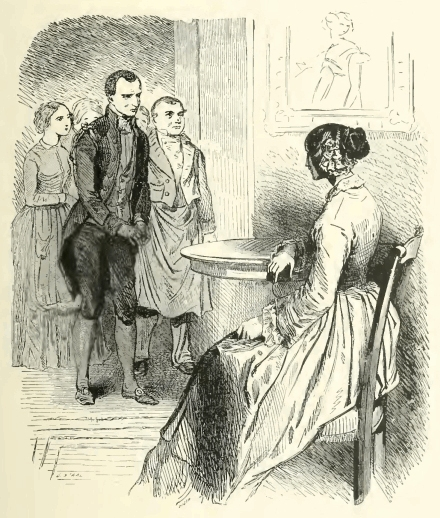
\includegraphics[width=\textwidth]{40124m.jpg}
\end{figure}

“Listen,” cried he; “pity me—help me! No, my daughter is not guilty. If
you drag us both before a tribunal I will still say, ‘No, my daughter
is not guilty;—there is no crime in my house. I will not acknowledge a
crime in my house; for when crime enters a dwelling, it is like
death—it does not come alone.’ Listen. What does it signify to you if I
am murdered? Are you my friend? Are you a man? Have you a heart? No,
you are a physician! Well, I tell you I will not drag my daughter
before a tribunal, and give her up to the executioner! The bare idea
would kill me—would drive me like a madman to dig my heart out with my
finger-nails! And if you were mistaken, doctor—if it were not my
daughter—if I should come one day, pale as a spectre, and say to you,
‘Assassin, you have killed my child!’—hold—if that should happen,
although I am a Christian, M. d’Avrigny, I should kill myself.”

“Well,” said the doctor, after a moment’s silence, “I will wait.”

Villefort looked at him as if he had doubted his words.

“Only,” continued M. d’Avrigny, with a slow and solemn tone, “if anyone
falls ill in your house, if you feel yourself attacked, do not send for
me, for I will come no more. I will consent to share this dreadful
secret with you, but I will not allow shame and remorse to grow and
increase in my conscience, as crime and misery will in your house.”

“Then you abandon me, doctor?”

“Yes, for I can follow you no farther, and I only stop at the foot of
the scaffold. Some further discovery will be made, which will bring
this dreadful tragedy to a close. Adieu.”

“I entreat you, doctor!”

“All the horrors that disturb my thoughts make your house odious and
fatal. Adieu, sir.”

“One word—one single word more, doctor! You go, leaving me in all the
horror of my situation, after increasing it by what you have revealed
to me. But what will be reported of the sudden death of the poor old
servant?”

“True,” said M. d’Avrigny; “we will return.”

The doctor went out first, followed by M. de Villefort. The terrified
servants were on the stairs and in the passage where the doctor would
pass.

“Sir,” said d’Avrigny to Villefort, so loud that all might hear, “poor
Barrois has led too sedentary a life of late; accustomed formerly to
ride on horseback, or in the carriage, to the four corners of Europe,
the monotonous walk around that armchair has killed him—his blood has
thickened. He was stout, had a short, thick neck; he was attacked with
apoplexy, and I was called in too late. By the way,” added he in a low
tone, “take care to throw away that cup of syrup of violets in the
ashes.”

The doctor, without shaking hands with Villefort, without adding a word
to what he had said, went out, amid the tears and lamentations of the
whole household. The same evening all Villefort’s servants, who had
assembled in the kitchen, and had a long consultation, came to tell
Madame de Villefort that they wished to leave. No entreaty, no
proposition of increased wages, could induce them to remain; to every
argument they replied, “We must go, for death is in this house.”

They all left, in spite of prayers and entreaties, testifying their
regret at leaving so good a master and mistress, and especially
Mademoiselle Valentine, so good, so kind, and so gentle.

Villefort looked at Valentine as they said this. She was in tears, and,
strange as it was, in spite of the emotions he felt at the sight of
these tears, he looked also at Madame de Villefort, and it appeared to
him as if a slight gloomy smile had passed over her thin lips, like a
meteor seen passing inauspiciously between two clouds in a stormy sky.
